% ==================================================
% CHAPTER 2: The LHC and ATLAS Experiment %
% ==================================================

\chapter{High energy particle physics at the LHC and the ATLAS experiment}
\label{chap:lhc_atlas}
% Edit count: Lia - 1, Brigitte - 0

The LHC, ATLAS, and the upgrades they are undergoing are all motivated by the study of the SM and the open questions the SM does not address. Particle physics aims to study the indivisible constituents of matter. Understanding the fundamental building blocks and how they interact informs our understanding of the evolution of the Universe from the Big Bang to the forms of matter we recognize today. This chapter provides context for the NSW upgrade. The study of particle physics using accelerators is introduced, before moving on to the LHC, HL-LHC and the ATLAS experiment. The connection to physics questions of interest will be highlighted at each stage. 

The information on particle physics and the SM presented here is rather general; the reader is referred to~\cite{griffiths_introduction_2011, peskin_introduction_1995, zyla_review_2020} for more information. 

\textcolor{red}{\textit{Do I need to place the background texts I cite in the in-text citations? I've listed where I've personally gotten each piece of information, but info about the SM and BSM might be so basic as to not required a citation. Comments?}}

% --------------------------------------------------
\section{The Standard Model}
% --------------------------------------------------

The SM describes all the fundamental particles and their interactions\iffalse[GRIFFITHS]\fi. It is a collection of quantum field theories able to explain the existence of all the particles discovered in the past century and predict how they interact to incredible precision\iffalse[PESKIN]\fi. In fact, when it was being developed in the 1960s-1970s, it began motivating the search for yet undiscovered particles, like the tau neutrino with DONUT in 2002~\cite{kodama_detection_2002}.

\begin{figure}
    \centering
    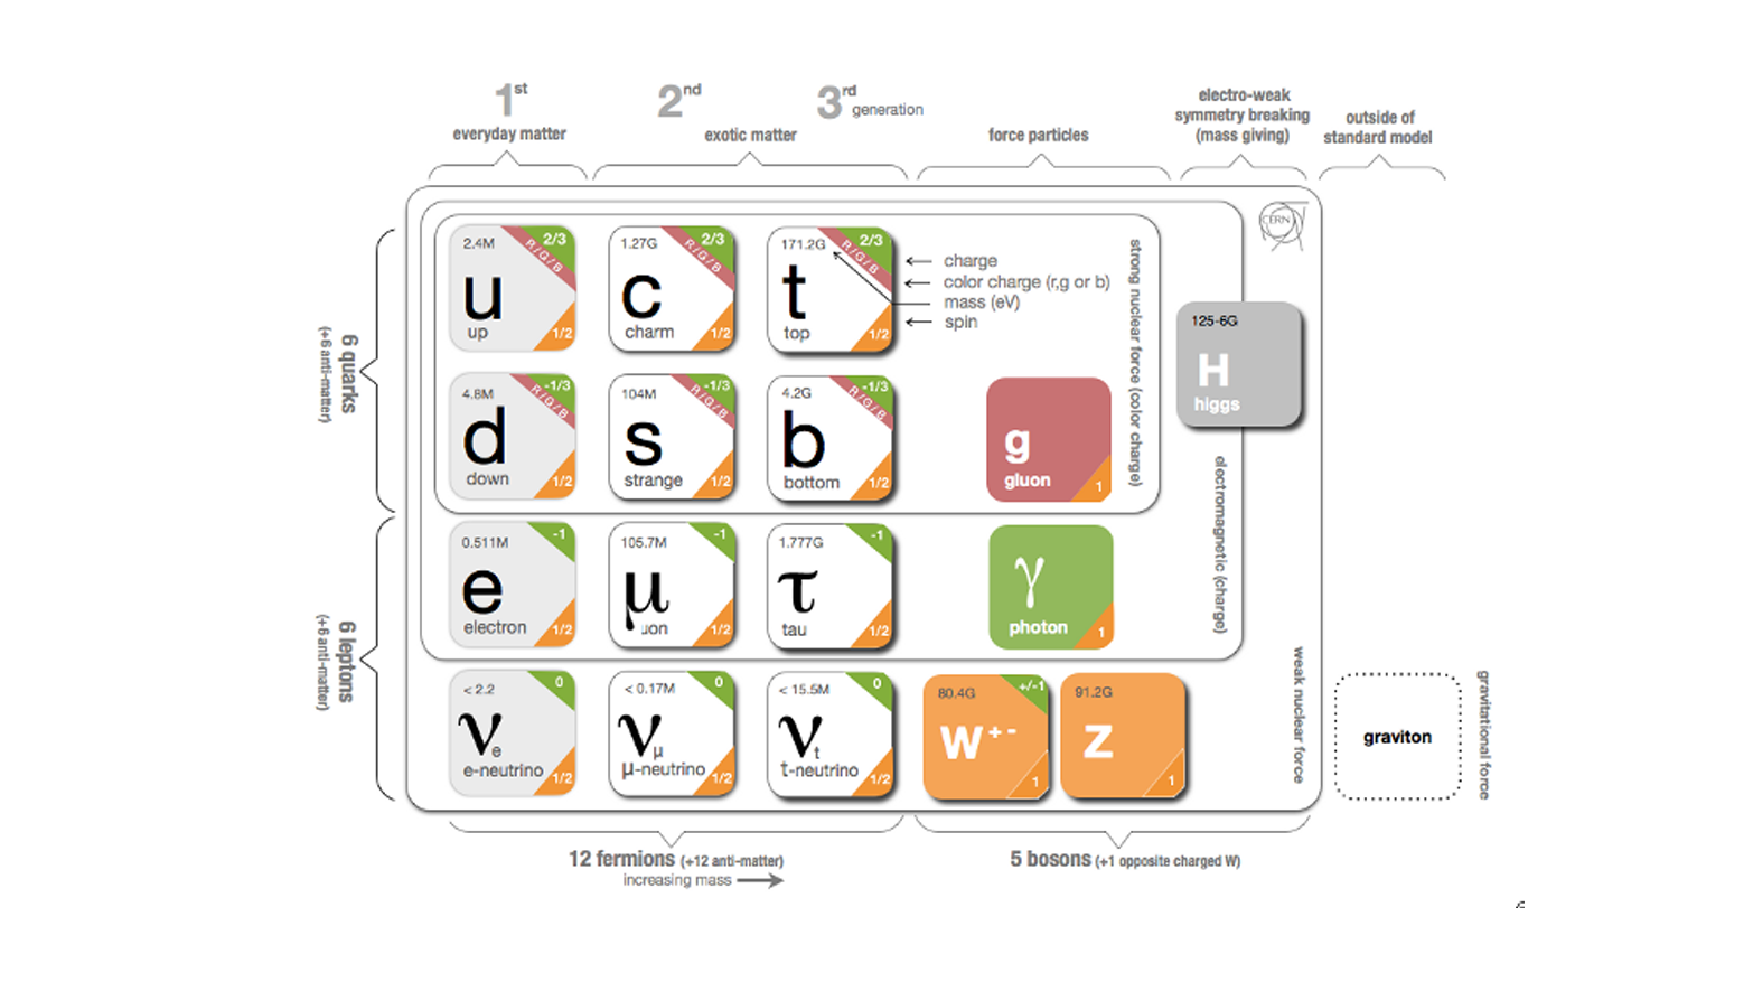
\includegraphics[width = \textwidth]{figures/standardmodel_galbraith_carsten.pdf}
    \caption{Representation of the SM of particle physics. There are three main types of particles: quarks, leptons and force-particles. The version highlights which groups of particles each force-particle interacts with. The force-particle in each black enclosure interacts with all quarks/leptons within the enclosure~\cite{galbraith_ux_2013}.}
    \label{fig:standard_model}
\end{figure}

The SM represented in figure~\ref{fig:standard_model}, consists of six quarks, six leptons, and five force-particles. Note that each particle also has an anti-particle, which are not represented. The force-carrying bosons are exchanged between interacting (coupled) particles to produce what is perceived as: the strong force mediated by gluons; the electromagnetic force mediated by photons; and the weak force mediated by the charged W-bosons and neutral Z-boson\iffalse[GRIFFITHS]\fi. The SM actually presents a theory of the electromagnetic and weak force as one force stemming from the same phenomenon: the unified electroweak force\iffalse[PESKIN]\fi. The Higgs boson field interacts with the particles mediating the unified electroweak force to distinguish the weak and electromagnetic forces from each other and give all particles (except neutrinos) a mass. This is called electroweak symmetry breaking\iffalse[PESKIN]\fi. 

Quarks are fermions that are sensitive to all forces; notably they are the only particles sensitive to the strong force\iffalse[GRIFFITHS]\fi. Protons and neutrons are made up of quarks and gluons, and the strong force is responsible for their existence and mutual attraction into nuclei~\cite{bertulani_nuclear_2007}. Leptons are particles not sensitive to the strong force. Charged leptons include the electron, which once part of atoms is responsible for chemistry. Neutrinos are neutral, almost massless particles that only interact through the weak force\iffalse[GRIFFITHS]\fi. 

Common matter is made up of the lightest constituents of the SM: up and down quarks, electrons and photons. The other particles are or were generated in high-energy environments and decay eventually to the lightest constituents. Such high energy environments include the Big Bang~\cite{carroll_introduction_2007}, astrophysical sources, and accelerators\iffalse[REV PART PHYS, GRIFFITHS]\fi. The presence of the particles of the SM at the beginning of the Universe means that their interactions and decays are fundamental for the study of the origin of the Universe~\cite{carroll_introduction_2007}. Many high energy astrophysical sources, like supernovae, generate particles that rain down on Earth as cosmic rays~\cite{boezio_chemical_2012}\iffalse[BOEZIO, REV PART PHYS, GRIFFITHS]\fi. Accelerators were built to create controlled, high energy and high rate environments where the production and decay of fundamental particles can be manufactured, detected and studied\iffalse[GRIFFITHS, REV PART PHYS]\fi.

% --------------------------------------------------
\section{Beyond the Standard Model}
% --------------------------------------------------

The SM provides no explaination for several open questions in particle physics.

First, gravity is not included in the SM. One might expect a force-particle to exist that mediates the gravitational force, but the strength of gravity is so weak that the ``graviton'' will elude detection for a long time. Moreover, there is no theory of gravity that does not require dark energy or dark matter~\cite{zyla_review_2020}. The universe is expanding at a rate irreconcilable with the known energy density of the Universe, and the nature of this ``dark energy'' is unknown~\cite{carroll_introduction_2007}. Similarly, dark matter is the name given to mass in the universe whose gravity is measurable, but for which there is no SM explanation~\cite{munoz_dark_2004}.

Second, neutrinos in the SM are massless; they do not interact with the Higgs field. However, in 2013 neutrino oscillations were confirmed, which can only occur if neutrinos do have mass~\cite{aharmim_combined_2013}.

Third, the unification of the electromagnetic and weak force begs the question of if there is a Grand Unified Theory (GUT) that includes the strong force and emcopasses the SM in a more complete theory~\cite{georgi_unity_1974}. 

Theories beyond the standard model (BSM) aim to answer these questions. Often, BSM theories predict new particles. For example, super-symmetry (SUSY) predicts that each SM particle has a heavier super-symmetric partner. SUSY would explain the origin of dark matter with weakly interacting massive particles, would solve the so-called "naturalness" problem in the SM at energies above the tera-electronvolt scale, and is often a part of GUTs~\cite{jungman_supersymmetric_1996}. Ideally, a BSM theory predicts a measurable signature that can be searched for at accelerators or elsewhere.

% --------------------------------------------------
\section{Studying high energy particle physics with accelerators}
% --------------------------------------------------

Accelerators of increasingly high energy have a long history of enabling the discovery of new particles\iffalse[GRIFFITHS]\fi. Only calling on one example, one of the main goals when the LHC, the ATLAS experiment and the CMS experiment were proposed was to detect the long-predicted Higgs boson particle~-- a triumph accomplished in 2012~\cite{the_atlas_collaboration_observation_2012, the_cms_collaboration_observation_2012}. Being the last particle of the SM to be discovered, the discovery marked the completion of the SM as it is known today.

Since then, measurements of the cross section of particle physics processes have been enabled by the LHC. A summary of the cross sections measurements done at the ATLAS experiment is shown in figure~\ref{fig:atlas_cross_sections}. Given the precision to which the SM predicts cross sections and the precision to which many can be measured, any discrepancy between theory and experiment could be an indication of new physics. The questions the SM does not address require new physics; searching for it at accelerators is a natural choice.

\begin{figure}
    \centering
    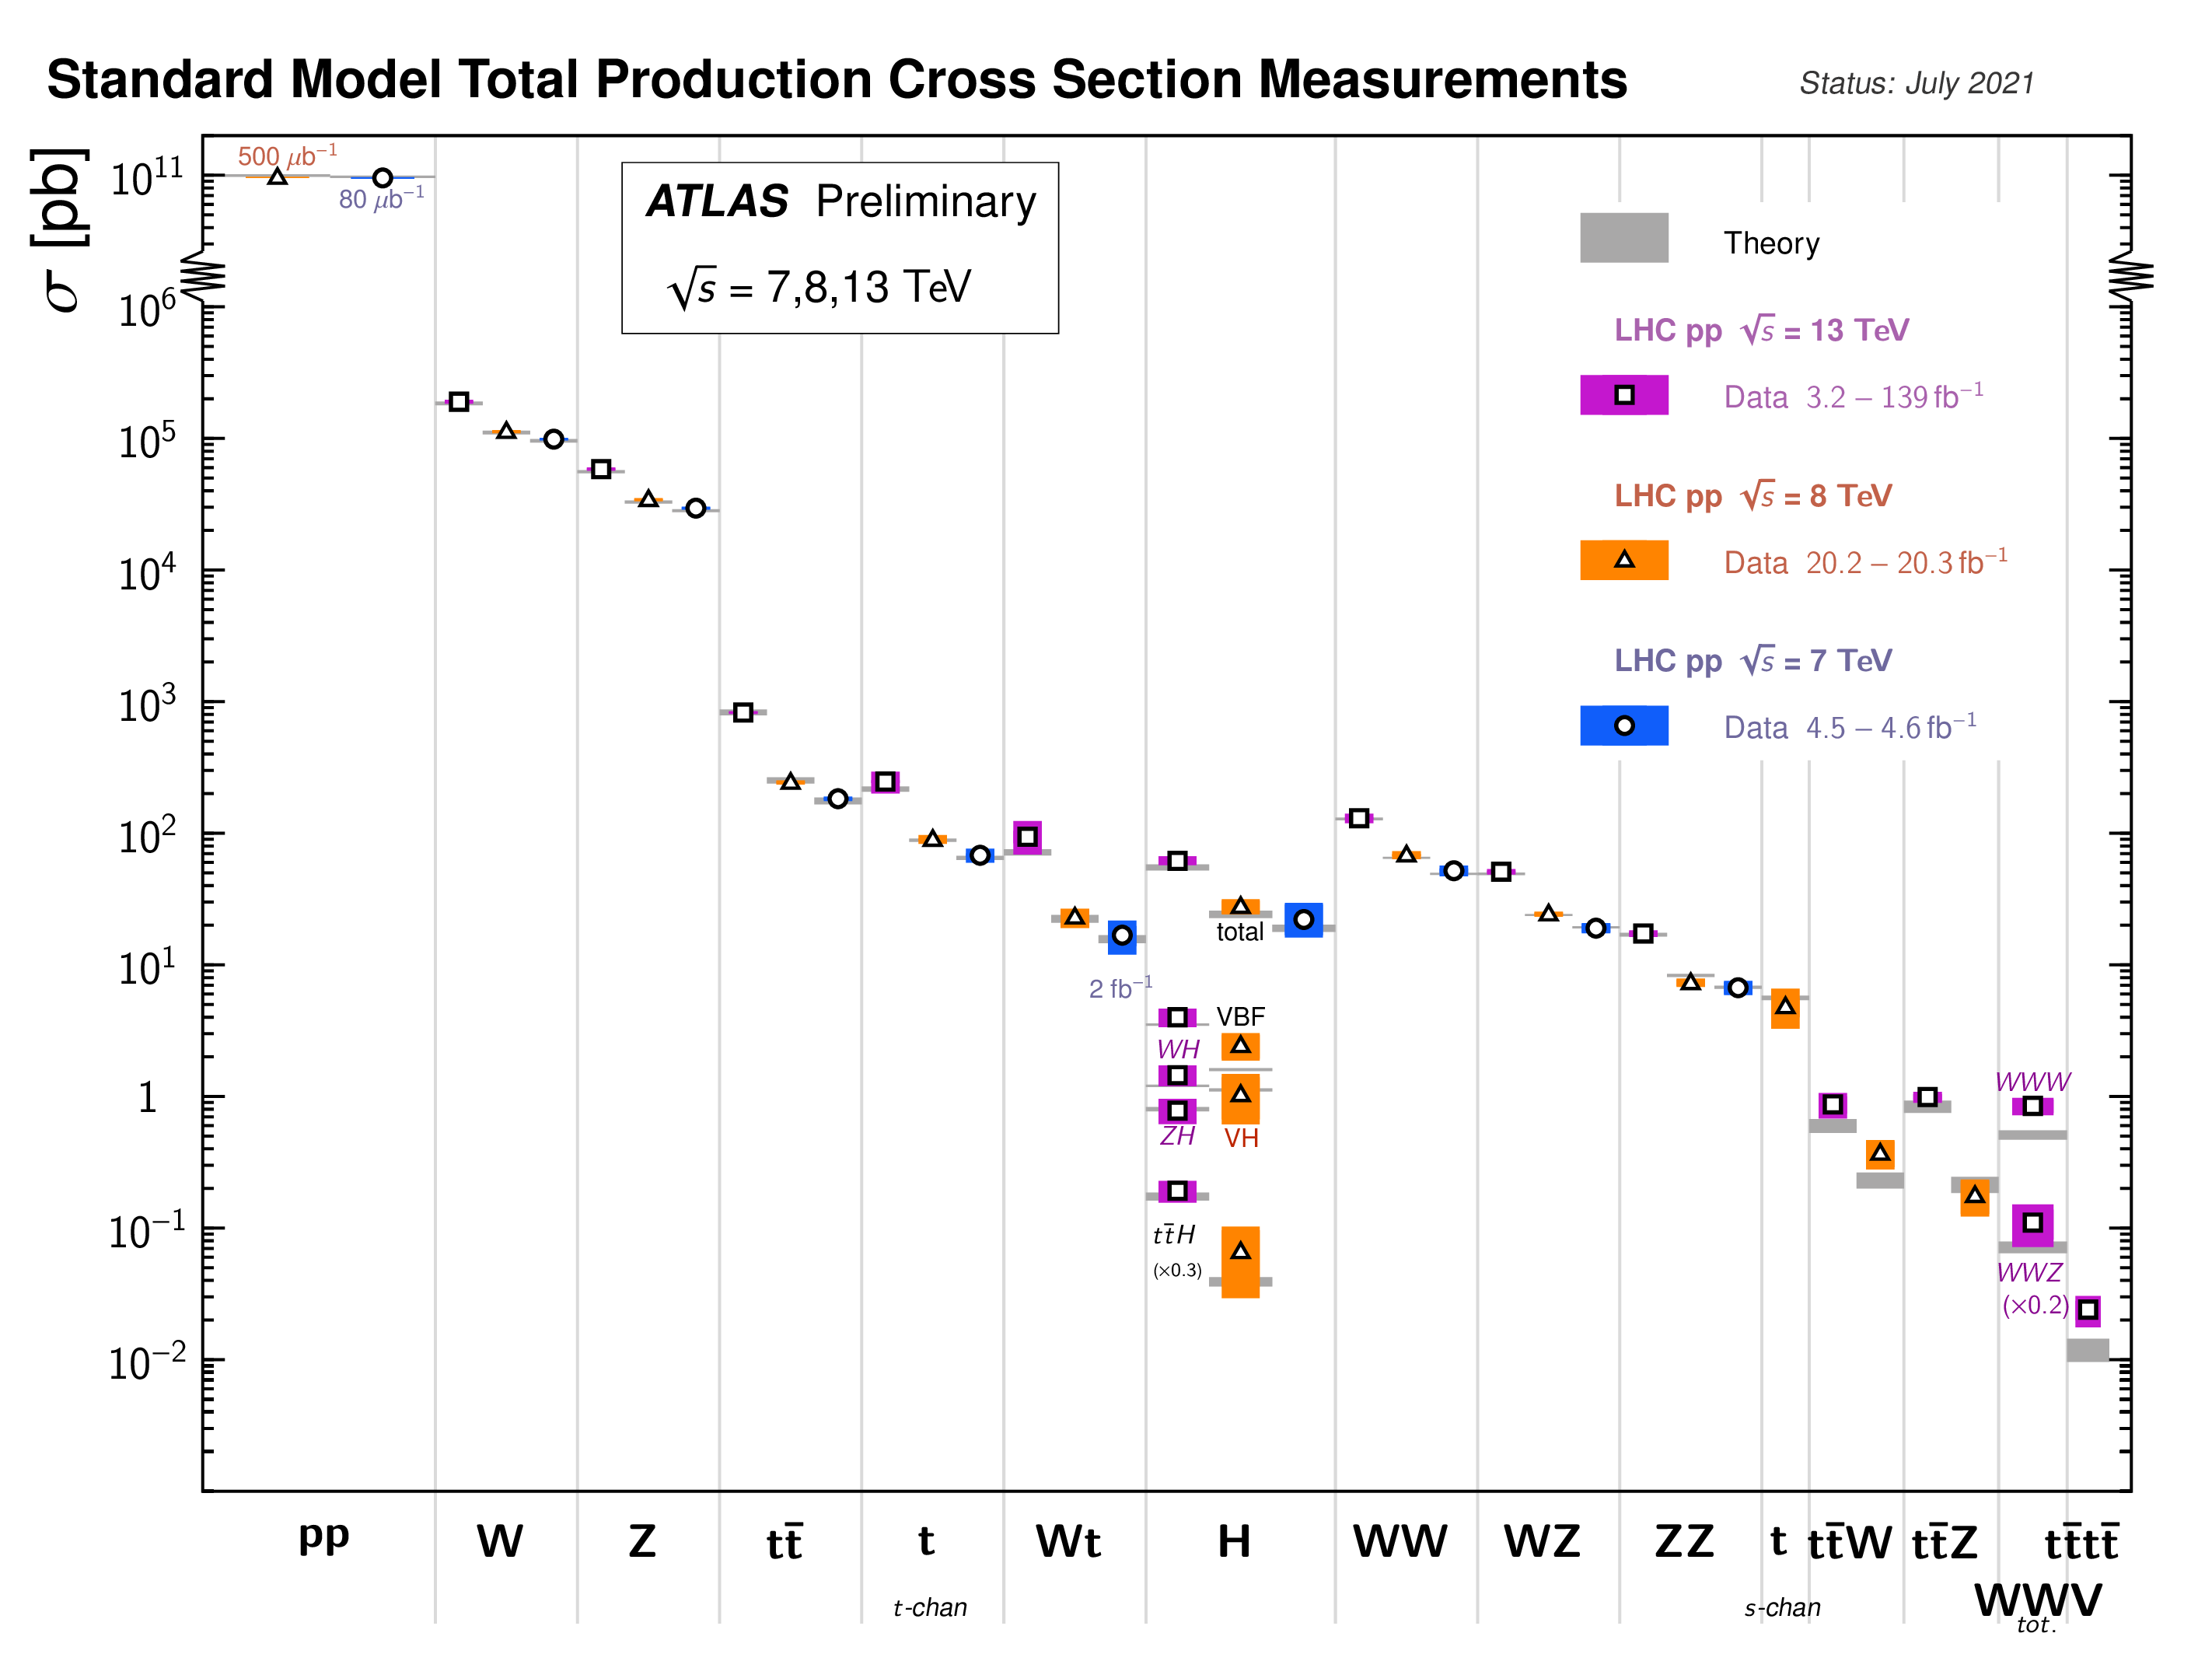
\includegraphics[width = \textwidth]{figures/atlas_cross_sections.png}
    \caption{Cross sections of select SM physics interactions measured using the ATLAS experiment at the LHC. The comparison with theoretical predictions is also shown~\cite{atlas_public_web_sm}.}
    \label{fig:atlas_cross_sections}
\end{figure}

Accelerators and detectors can also be used to search for signatures of rare processes predicted by the SM and BSM theories. The controlled, high rate environment enables the search for signatures that would be impossible to discern in other environments. If the signature is not found, exclusion limits can be set~\cite{lista_statistical_2017}.

Through measurements and searches, accelerators play a key role in making precision measurements, searching for rare processes predicted by the SM, and testing BSM theories.

\textcolor{red}{\textit{Is there a good citation for the defintion of search vs measurement?}}

% --------------------------------------------------
\section{The Large Hadron Collider}
% --------------------------------------------------

% Include order for inst lum.
% Include bunch crossing frequency
The LHC is an accelerator \SI{27}{\kilo\meter} in circumference and located $\sim$\SI{100}{\meter} underground at CERN near Geneva, Switzerland~\cite{evans_lhc_2008}. It has two beam pipes that counter-circulate bunches of protons\footnote{the LHC also accelerates lead ions, but ATLAS is best at recording proton-proton collisions. The ALICE experiment~\cite{alice_2008} was designed for lead-lead interactions.} before colliding the bunches in the center of one of four major experiments, such as the ATLAS experiment (discussed in section~\ref{sec:atlas}). In the previous run of the LHC (run-2), protons were collided with a center of mass energy of \SI{13}{\tera\electronvolt}. It is not actually the protons that interact, but the constituent quarks and gluons (partons) that each carry some fraction of the energy and momentum of the collisions.

% There are two main branches of study that can be pursued with the LHC and ATLAS. First, properties predicted by the standard model (SM) of particle physics can be measured. Else, physicists can search for evidence of processes predicted by theories beyond the standard model. Both the SM measurement and search analyses are based on measuring the number of times a given process occurs and comparing it to expectations. In this way, the number of proton-proton interactions created by the LHC directly affects the statistics available to do SM measurements and searches using the ATLAS experiment.

% --------------------------------------------------
\section{Luminosity}
% --------------------------------------------------

The number of proton-proton interactions generated by the LHC directly affects the statistics available to make measurements of cross sections, SM parameters, etc. 
%IF YOU DON'T NEED TO DEFINE LUMINOSITY
% The number of interactions is quantified by luminosity, a property of the accelerator and its operating conditions~\cite{zyla_review_2020}. When the instantaneous luminosity is integrated over a data collection period and multiplied by the cross section of a given process, the result is the expected number of times that process occurs (so luminosity has units of inverse cross section). Since luminosity is derived from the accelerator parameters, it is the link between the machine and the statistical power of potential measurements. 
% IF YOU NEED TO DEFINE LUMINOSITY
% THIS SECTION IS NOT CITED, probably cite wiht zyla_review_2020
Predicting the number of proton-proton interactions requires defining a metric called luminosity~\cite{zyla_review_2020}. It is the number of particles an accelerator can send through a given area per unit time. It is calculated from the measurable quantities in equation~\ref{eqn:inst_lum}:

\begin{equation}
\mathcal{L} = \frac{f N_{1} N_{2} }{4 \pi \sigma_{x} \sigma_{y}}
\label{eqn:inst_lum}
\end{equation}

$f$ is the frequency of the bunch crossings (\SI{25}{\nano\second}), $N_{1}$ and $N_{2}$ are the number of protons in each bunch ($\sim 10^{11}$ protons / bunch), and $\sigma_{x}$ and $\sigma_{y}$ are the RMS of the spatial distributions of the bunch. Therefore, luminosity is a property of accelerator beams, which are set by the capabilities of the accelerator. The design luminosity of the LHC was $10^{34}$ cm$^{-2}$s$^{-1}$. The units of luminosity are an inverse area; multiplying the luminosity by the cross section of a given process gives the expected rate for that process.

Integrating the \textit{instantaneous} luminosity (equation~\ref{eqn:inst_lum}) over a period of data collection gives the integrated luminosity,

\begin{equation}
L = \int \mathcal{L} \left( t \right) \,dt
\label{eqn:int_lum}
\end{equation}

which is related to the total number of interactions. In this way, the luminosity is the link between the accelerator and the statistical power of measurements to be made with the data collected. So far, the LHC provided an integrated luminosity of \SI{28.26}{\per\femto\barn} in run-1~\cite{atlas_luminosity_run1} and \SI{156}{\per\femto\barn} in run-2~\cite{atlas_luminosity_run2}.

% --------------------------------------------------
\section{The High-luminosity LHC}
% --------------------------------------------------

The HL-LHC upgrade~\cite{hl_lhc_tdr} was accepted because without increasing the luminosity of the LHC tenfold, running the accelerator will not provide significant statistical gain on measurements. Also, some systems will need repair and replacement to operate past $\sim$2020. The LHC will be the most energetic accelerator in the world for years to come and is the only accelerator capable of directly producing the Higgs boson (and top quarks), so the European Strategy for Particle Physics made it a priority ``to fully exploit the physics potential of the LHC'' with ``a major luminosity upgrade''~\cite{european_strategy_for_particle_physics}. The goal is for the HL-LHC to provide an integrated luminosity of \SI{3000}{\per\femto\barn} in the 12 years following the upgrade. The luminosity actually achieved will depend on a combination of technological advances and upgrades in progress that affect the factors contributing to luminosity defined in equation~\ref{eqn:inst_lum}~\cite{hl_lhc_tdr}.

\begin{figure}
    \centering
    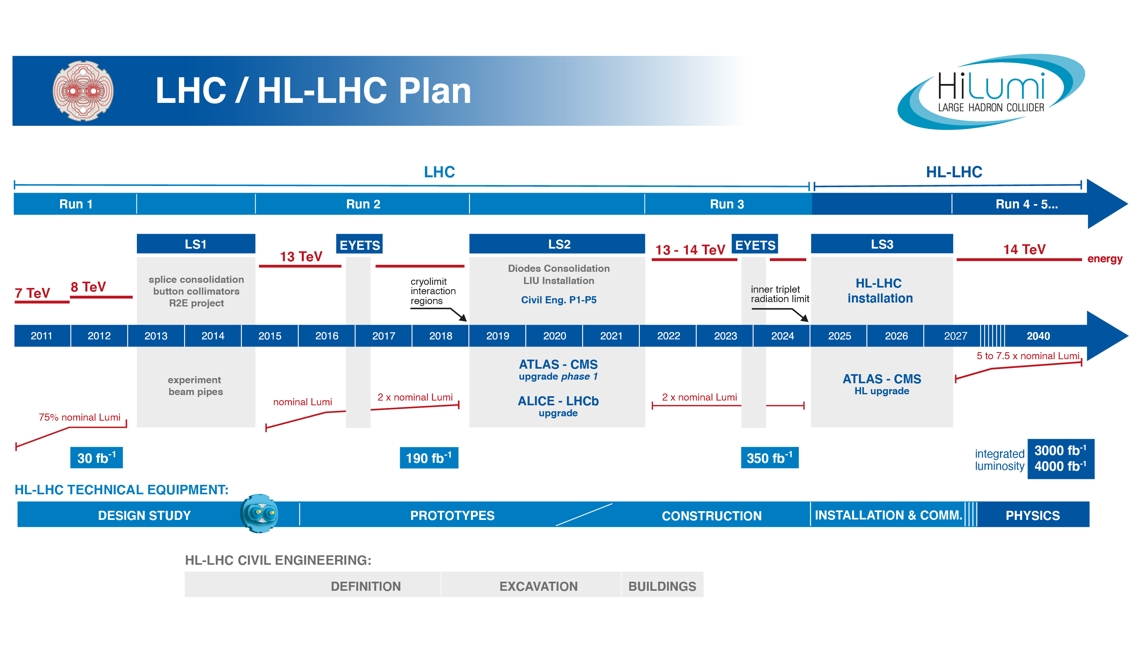
\includegraphics[width = \textwidth]{figures/HL-LHC-updated-January-2021_small.jpg}
    \caption{LHC/HL-LHC plan~\cite{hl-lhc_plan_picture_website}. The integrated luminosities collected and projected for each run of the LHC are shwon in blue boxes below the timeline and the center of mass energy of the collisions is shown in red above the timeline. The top blue arrow labels the run number. ``LS'' stands for ``long shutdown'' and indicates periods where the accelerator is not operating. During the shutdowns, upgrades to the LHC and the experiments are being installed. This timeline was last updated in January, 2021, and reflects changes in the schedule due to the ongoing pandemic. }
    \label{fig:hl-lhc}
\end{figure}

% The increase in statistics the HL-LHC will improve measurements of standard model parameters and improve searches for unobserved phenomena~\cite{dainese_physics_2018}. A particular measurement that will benefit from the increased statistics is of the triple-Higgs coupling. Measuring the coupling measures the shape of the Higgs potential responsible for electroweak symmetry breaking. Any discrepancy with the SM prediction will show that there must be other sources of electroweak symmetry breaking~-- if there is such another source, it could be an avenue to study the other questions the SM does not address. Also, the sensitivity to several exotic Higgs decays to BSM particles will be improved. Many of the products of exotic Higgs decays are dark matter candidates or otherwise could extend the scope of the SM.

% Higgs couplings to particles will all be measured to the percent level at the HL-LHC and sensitivity to SM predicted Higgs decays will increase. Also, the sensitivity to several exotic Higgs decays to BSM particles will be improved. Many of the products of exotic Higgs decays are dark matter candidates or otherwise could extend the scope of the SM. The LHC is the only accelerator energetic enough to directly produce Higgs bosons, so it is the only tool able to probe questions about the Higgs.

The most anticipated measurement at the HL-LHC is of the triple-Higgs coupling. Measuring the coupling allows the shape of the Higgs potential responsible for electroweak symmetry breaking to be measured. Any discrepancy with the SM prediction will show that there must be other sources of electroweak symmetry breaking, and hence currently unpredicted particles. The LHC is the only accelerator where the Higgs can be produced directly and the HL-LHC upgrade is required to have sufficient di-Higgs production to make a meaningful measurement~\cite{dainese_physics_2018, cepeda_report_2018}. Accordingly, detector sensitivity to various Higgs decays will be important at the HL-LHC.
%The estimated number of interactions of a given type per bunch crossing is given by equation~\ref{eqn:num_interactions}.
%\begin{equation}
%\mu = \sigma \delta t\mathcal{L}
%\label{eqn:num_interactions}
%\end{equation}

% The energies accessible by the accelerator make it unique infrastructure with which to study processes of the standard model of particle physics and search for new phenomenon beyond the standard
% model. Considerable progress has been made towards answering the questions originally used to motivate the construction of the LHC, but many remain unanswered or only partially answered~ \cite{brianti_large_1984}. Therefore, the continued use and maintenance of the accelerator 

% --------------------------------------------------
\section{The ATLAS experiment}
% --------------------------------------------------
\label{sec:atlas}

The ATLAS experiment~\cite{collaboration_atlas_2008} was designed to support all the physics goals of the LHC. It is \SI{44}{\meter} long and \SI{25}{\meter} in diameter, and weighs 7000 tones. It is an array of particle detector subsystems arranged concentrically around the beam pipe and centered around one of the LHC's interaction points (a place where the beams collide), as shown in figure~\ref{fig:atlas}. ATLAS is cylindrical because it aims to provide 4$\pi$ coverage around the interaction point. It is helpful to separate the subsystems of ATLAS into the so-called ``barrel'' and ``endcap''/``forward'' regions, referring to the cylindrical geometry. 

\begin{figure}
    \centering
    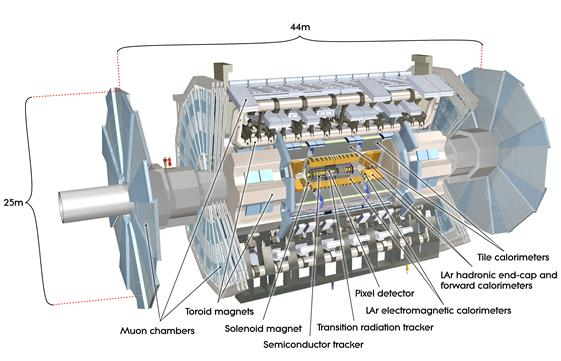
\includegraphics[width = \textwidth]{figures/atlas_diagram.png}
    \caption{Diagram of the ATLAS experiment, with the various detector subsystems labelled~\cite{collaboration_atlas_2008}.}
    \label{fig:atlas}
\end{figure}

For analysis, ATLAS is typically described in spherical coordinates. The azimuthal angle $\phi$ is measured around the beampipe and the polar angle $\theta$ is measured from the beam pipe. A more useful coordinate than $\theta$ is the pseudo-rapidity, $\eta = -\ln\tan\left(\theta/2\right)$, because it approaches the rapidity of a particle when its momentum is much greater than its mass and differences in rapidity are approximately invariant to a Lorentz boost parallel to the beam. The range of $\eta$ is 0 (perpendicular to the beam) to $\pm\infty$ (parallel to the beam, or the z-direction). Typically, $\eta$ is the physically interesting coordinate because the $\phi$ coordinate follows the cylindrical symmetry of the beam.

ATLAS provides identification and kinematic measurements for each particle created after the initial collision. Predictions made using SM and BSM theories can then be compared to the data. Each subsystem of ATLAS collections certain information and a complete description of each recorded collision can be assembled offline. An overview of the main ATLAS subsystems is given below.

\paragraph*{The inner detector} \hfill \break
The inner detector~\cite{atlas_inner_detector_tdr_1, atlas_inner_detector_tdr_2} (figure~\ref{fig:atlas_inner_detector}) is for precision tracking, vertex measurements and electron identification. A \SI{2}{\tesla} solenoid with field parallel to the beam bends the track of outgoing particles. The innermost part is made of high-resolution semiconductor pixel and strip detectors while the outermost part are straw-tubes that generate and detect transition radiation

\begin{figure}
    \centering
    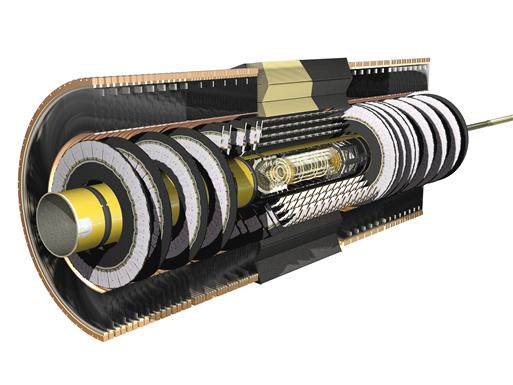
\includegraphics[width = 0.5\textwidth]{figures/atlas_inner_detector.jpg}
    \caption{Diagram of the ATLAS experiment's inner detector, with the different segments and the technology used labelled~\cite{collaboration_atlas_2008}.}
    \label{fig:atlas_inner_detector}
\end{figure}

\paragraph*{Calorimetry system} \hfill \break
Electromagnetic and hadronic sampling calorimeter units are used to record the energy of electrons, photons and jets. A combination of liquid-argon (LAr) electromagnetic and hadronic calorimeters~\cite{atlas_lar_cal_tdr} and tile-scintillator hadronic calorimeters~\cite{atlas_tile_cal_tdr} cover the rapidity range $|\eta| < 4.9$, as shown in figure~\ref{fig:atlas_calorimeter}.

\begin{figure}
    \centering
    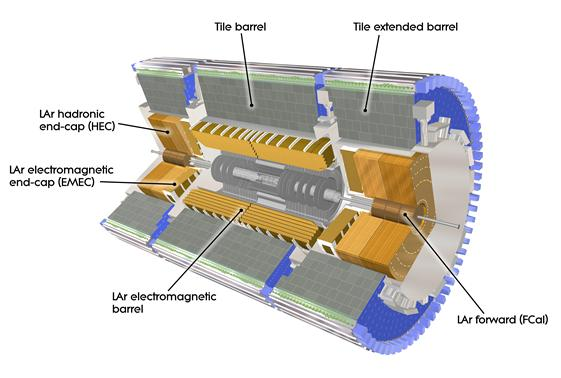
\includegraphics[width = 0.5\textwidth]{figures/atlas_calorimeter.png}
    \caption{Diagram of the ATLAS calorimeter system, with the different segments and the technology used labelled~\cite{collaboration_atlas_2008}.}
    \label{fig:atlas_calorimeter}
\end{figure}

The calorimeters cause incoming charged particles to shower and deposit their energy in the sensitive volume. Only muons and neutrinos are known to pass the calorimeters to the muon spectrometer.  Particles other than those mentioned would have decayed in the inner detector before reaching the calorimeter. 

\paragraph*{Trigger system} \hfill \break
It would be impossible to record all the data from bunch crossings every \SI{25}{\nano\second}, corresponding to a rate of $\sim$\SI{40}{MHz}. ATLAS has a multi-level trigger system to select events of interest for permanent storage. The Level-1 (L1) hardware trigger~\cite{atlas_l1_trigger_tdr} uses partial-granularity information from the muon spectrometer and calorimeter to trigger on high $p_T$ muons, electrons, jets, high missing transverse energy, and $\tau$ decaying to hadrons. The maximum L1 trigger rate ATLAS can accommodate is \SI{100}{kHz} with a latency of \SI{2.5}{\micro\second}. After run-3 an upgrade of the trigger system will allow for a higher rate and more latency, but for now these are the working limits~\cite{tdaq_phase2_tdr}.

% The Level-1 (L1) hardware trigger uses the muon spectrometer's TGCs and RPCs to trigger on high $p_T$ muons and the calorimeter detector units to trigger on electrons, jets, high missing transverse energy, and $\tau$ decaying to hadrons, with a maximum trigger rate of \SI{100}{kHz} and latency of \SI{2.5}{\micro\second}. The L1 trigger only uses a fraction of the granularity offered by the detectors.

The L1 trigger is used to define regions of interest that are fed into the software high level trigger (HLT), in which the full granularity of the muon spectrometer and calorimeter are used with information from the inner detector to reduce the trigger rate to 1 kHz. Events that pass the L1 and HLT trigger are recorded for use in offline analysis~\cite{atlas_hlt_trigger_tdr}.

The ATLAS trigger system is described in the references above but the trigger rates quoted here are after the upgrades implemented for run-2, described in~\cite{martinez_run-2_2016}.

\paragraph*{Muon spectrometer} \hfill \break
The muon spectrometer has multiple layers, each of which records the position of a passing muon. Magnetic deflection by superconducting air-core toroid magnets bend the muon tracks. The position information recorded in each layer and the magnetic field are used to reconstruct each muon's momentum. In the barrel of ATLAS, eight coils bent into ``racetracks'' arranged around the beampipe provide the magentic field. In the forward region, two end-cap toroids each with eight smaller racetrack-shaped coils arranged symmetrically around the beampipe are inserted in the ends of the barrel toroid~\cite{atlas_magnet_tdr}. Figure~\ref{fig:atlas_muon_spectrometer} shows the toroid magnets and the different parts of the ATLAS muon spectrometer~\cite{collaboration_atlas_2008}.

\begin{figure}
\centering
\begin{subfigure}{.5\textwidth}
  \centering
  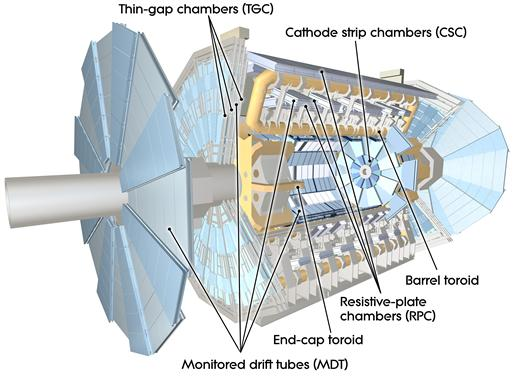
\includegraphics[width=\linewidth]{figures/atlas_muon_spectrometer.jpg}
  \caption{}
  \label{fig:atlas_muon_spectrometer_3D}
\end{subfigure}%
\begin{subfigure}{.5\textwidth}
  \centering
  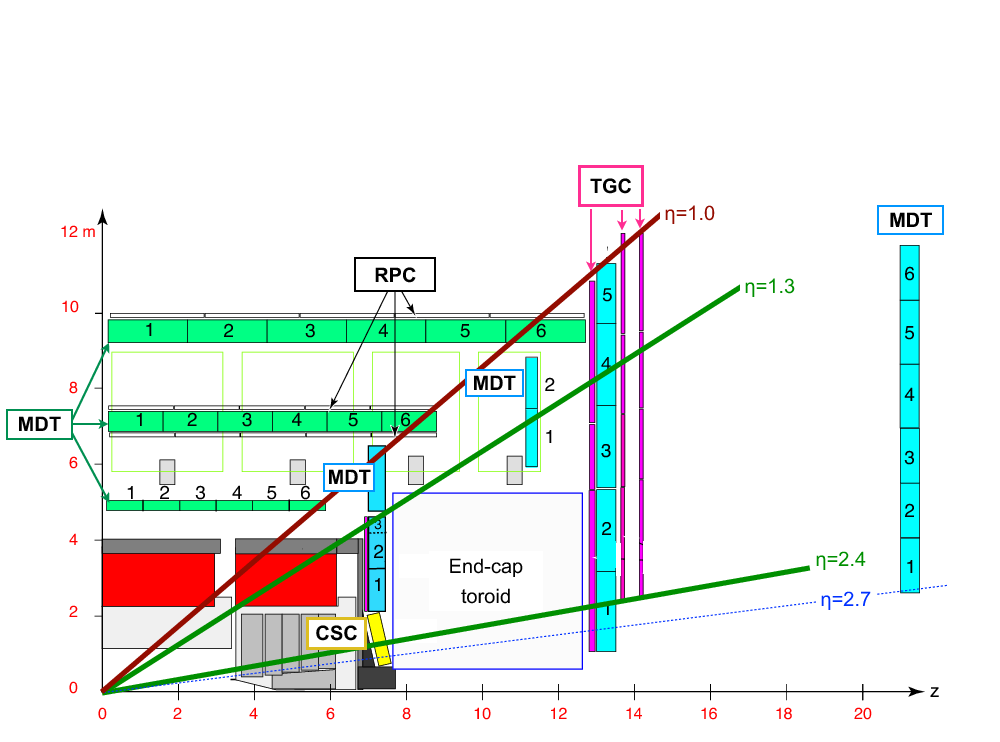
\includegraphics[width=\linewidth]{figures/atlas_old_muon_spec_quarter_cut_recolour.png}
  \caption{}
  \label{fig:atlas_muon_spectrometer_cut}
\end{subfigure}
\caption{(a) The ATLAS muon spectrometer~\cite{collaboration_atlas_2008}. (b) A quarter-cut of ATLAS, with the interaction point in the bottom left corner. The small wheel is just left of the end cap toroid, the big wheel is to its right, and the outer wheel is the rightmost structure~\cite{atlas_performance_muon_trigger_2015}.}
\label{fig:atlas_muon_spectrometer}
\end{figure}

The muon spectrometer~\cite{atlas_muon_spectrometer_tdr} is separated into detectors used for precision offline tracking and for triggering. Three layers of monitored drift tubes (MDTs) or cathode strip chambers (CSCs) are used for tracking. The position of the muon track in each of the three layers allows reconstruction of the track and hence momentum. For the design momentum resolution of $\Delta p_T / p_T <$~1$\times$10$^{-4}~p$~/~GeV for $p_T <$~300~GeV and a few percent for lower $p_T$ muons, the MDTs and CSCs required position resolution of \SI{50}{\micro\meter} each. Accordingly, an optical alignment system was designed to monitor and correct for chamber positions~\cite{atlas_muon_spectrometer_tdr, aefsky_optical_2008}. 

% Precision tracking is done offline for events passing the muon trigger. Each of the barrel and encap systems have three layers of MDTs that record the position of the muon as it passes through each layer. Knowing the magentic field, the muon's momentum can be extracted. For the design momentum resolution of $\Delta p_T / p_T <$ 1$\times$10$^{-4}~p$ / GeV for $p_T < 300 GeV$ and a few percent for lower $p_T$ muons, the MDTs and CSCs required position resolution of \SI{50}{\micro\meter} each. Accordingly, an optical alignment system was designed to monitor and correct for chamber positions~\cite{atlas_muon_spectrometer_tdr, aefsky_optical_2008}. 

% ON MUON TRIGGERING IN THE ENDCAP
% Decide how you want to do this based on the next section.
% At least 2 TGC layers in coincidence comes from muon spectrometer TDR; coincidence with "forward inner" detectors (small wheel) comes from run 2 trigger upgrades paper, Martinez.
% NSW TDR says there are TGC layers in the small wheel that are the forward inner detectors added to run 2 triggering.
% \textcolor{red}{The run 2 L1 muon trigger was passed if TGC layers (two for low $p_T$ muons, three for high $p_T$ muons) of the big wheel fired in coincidence with a hit from the MDTs of the small wheel on the order of the bunch crossing time. The regions of interest defined by the TGCs were fed into the HLT, where MDT and TGC data could be combined for further cuts. The $p_T$ resolution of the L1 trigger is improved by the MDT tracking information. \textit{I'll decide how I want to do this after writing the motivation for the NSW}}
Resistive plate chambers (RPCs) are used for triggering in the barrel and thin-gap chambers (TGCs) are used for triggering in the endcaps. The positions of each type of chamber are sketched in figure~\ref{fig:atlas_muon_spectrometer_cut}. Often, the endcap muon spectrometer is separated into three wheels~-- the small wheel, big wheel, and outer wheel~-- ordered by proximity to the interaction point. In run-1, low (high) $p_T$ muons were triggered on at L1 if two (three) of the RPCs or TGCs layers around the big wheel fired in coincidence, for the barrel and endcaps respectively~\cite{atlas_l1_trigger_tdr}. After run-1 it was discovered that up to 90\% of the triggers in the endcap were fake, caused by background particles generated in the material between the small wheel and the big wheel~\cite{nsw_tdr}.  To reduce the fake rate in run-2, the TGCs on the inside of the small wheel also had to register a hit. The added condition reduced the trigger rate by 50\% in the range 1.3 $< |\eta| <$ 1.9~\cite{martinez_run-2_2016}. The effectiveness of the solution was limited since the $|\eta|$-range of the small wheel TGCs was limited to 1.0 $< |\eta| <$ 1.9 and the position resolution of the small wheel TGCs is coarse~\cite{nsw_tdr}.

% In the barrel, three layers of MDTs are used for precision tracking, and resistive plate chambers (RPCs) are used for triggering. The endcaps of the muon spectrometer are composed of three wheels each, the small wheel (SW), big wheel, and outer wheel. All three wheels use MDTs for precision offline tracking, but cathode strip chambers (CSCs) are used in the forward region of the small wheel because they can better handle the increased background. Thin gap  chambers

% The big wheel and the outer wheel have MDTs for offline precision tracking and the thin gap chambers (TGCs) on either side for triggering. In the first two runs of ATLAS, offline precision tracking on the small wheel was done with MDTs and cathode strip chambers (CSCs), and their output did not contribute to the trigger.~\cite{atlas_muon_spectrometer_tdr}. 

% Sentences if you go without 1/4 cut figure
% In the barrel, three layers of monitored drift tubes (MDTs) are arranged between, above and below the barrel toroid magnets. They are used for precision tracking. On both sides of the middle layer of  MDTs and on the top of the top layer of MDTs are resitive plate chambers (RPCs), used for triggering.
%  The inner part had cathode strip chambers (CSCs), which had higher granularity to handle the increased background radiation rate in the forward region

% The muon spectrometer is the outermost layer of the ATLAS detector, since only muons (and neutrinos) can pass through the calorimeters. For muons that are ejected towards the end-caps of ATLAS, their trajectory is bent by the magentic field and their position recorded by three successive wheels of muon detectors. With each wheel providing the position of the muon along its trajectory and knowledge of the magentic field, the momentum of the muon generated in the collision can be reconstructed. 